\documentclass[CJK]{beamer}
\usepackage{CJKutf8}
\usepackage{beamerthemesplit}
\usetheme{Malmoe}
\useoutertheme[footline=authortitle]{miniframes}
\usepackage{amsmath}
\usepackage{amssymb}
\usepackage{graphicx}
\usepackage{color}
\usepackage{slashed}
\usepackage{simplewick}
\graphicspath{{../figures/}}
\def\be{\begin{equation}}
\def\ee{\nonumber\end{equation}}
\def\bea{\begin{eqnarray}}
\def\eea{\nonumber\end{eqnarray}}
\def\ii{{\dot{\imath}}}
\def\bch{\begin{CJK}{UTF8}{gbsn}}
\def\ech{\end{CJK}}
\def\bex{\begin{minipage}{0.3\textwidth}
\includegraphics[width=1in]{jugelizi.png}\end{minipage}\begin{minipage}{0.6\textwidth}}
\def\eex{\end{minipage}}
\def\chtitle#1{\frametitle{\bch#1\ech}}
\def\skipline{{\vskip0.1in}}
\def\skiplines{{\vskip0.2in}}
\def\lagr{{\mathcal{L}}}
\def\hamil{{\mathcal{H}}}
\def\vecv{{\mathbf{v}}}
\def\vecx{{\mathbf{x}}}
\def\veck{{\mathbf{k}}}
\def\vecp{{\mathbf{p}}}
\def\vecn{{\mathbf{n}}}
\def\vecA{{\mathbf{A}}}
\def\vecP{{\mathbf{P}}}
\def\vecsigma{{\mathbf{\sigma}}}
\def\hatJn{{\hat{J_\vecn}}}
\def\hatJx{{\hat{J_x}}}
\def\hatJy{{\hat{J_y}}}
\def\hatJz{{\hat{J_z}}}
\def\hatj#1{\hat{J_{#1}}}
\def\hatphi{{\hat{\phi}}}
\def\hatq{{\hat{q}}}
\def\hatpi{{\hat{\pi}}}
\def\vel{\upsilon}
\def\Dint{{\mathcal{D}}}
\def\adag{{\hat{a}^\dagger}}
\def\bdag{{\hat{b}^\dagger}}
\def\cdag{{\hat{c}^\dagger}}
\def\ddag{{\hat{d}^\dagger}}
\def\hata{{\hat{a}}}
\def\hatb{{\hat{b}}}
\def\hatc{{\hat{c}}}
\def\hatd{{\hat{d}}}
\def\hatN{{\hat{N}}}
\def\hatH{{\hat{H}}}
\def\hatp{{\hat{p}}}
\def\Fup{{F^{\mu\nu}}}
\def\Fdown{{F_{\mu\nu}}}
\def\newl{\nonumber \\}
\def\SIkm{\mathrm{km}}
\def\SIyr{\mathrm{yr}}
\def\SIGyr{\mathrm{Gyr}}
\def\SIeV{\mathrm{eV}}
\def\SIGeV{\mathrm{GeV}}
\def\SIm{\mathrm{m}}
\def\SIcm{\mathrm{cm}}
\def\SIJ{\mathrm{J}}
\def\SIs{\mathrm{s}}
\def\SIkg{\mathrm{kg}}
\def\SIg{\mathrm{g}}
\def\vece{\mathrm{e}}
\def\bmat#1{\left(\begin{array}{#1}}
\def\emat{\end{array}\right)}
\def\bcase#1{\left\{\begin{array}{#1}}
\def\ecase{\end{array}\right.}
\def\calM{{\mathcal{M}}}
\def\calT{{\mathcal{T}}}
\def\calR{{\mathcal{R}}}
\def\barpsi{\bar{\psi}}
\def\baru{\bar{u}}
\def\barv{\bar{\upsilon}}
\def\bmini#1{\begin{minipage}{#1\textwidth}}
\def\emini{\end{minipage}}
\def\qeq{\stackrel{?}{=}}
\def\torder#1{\mathcal{T}\left(#1\right)}
\def\rorder#1{\mathcal{R}\left(#1\right)}


\title{Quantum Field Theory I \\ Openmind Homework}
  \author{}
  \date{}


\begin{document}

\begin{frame}
 
\begin{center}
\begin{Large}
\bch
量子场论 I 

{\vskip 0.3in}

脑洞大开作业参考解答

\ech
\end{Large}
\end{center}

\vskip 0.2in

\bch
课件下载
\ech
https://github.com/zqhuang/SYSU\_QFTI

\end{frame}


\begin{frame}
\chtitle{第1题 二维空间的Casimir力}
\bch
\small{假设“脑洞大开世界”是2维空间加1维时间的平直时空,时空度量元为
$$ds^2 = (dx^0)^2 - (dx^1)^2-(dx^2)^2$$
在这个世界里的“脑洞大开人”发现真空中的相距为$d$的很长的(长度$\gg d$)两根平行金属线之间有大小为$F$的相互作用力,他们认为这是两条金属线之间的真空能的改变引起的作用力,并把这种力称为Casimir力。现在问,当把金属线之间的距离变为$d/2$,Casimir力变为多大?}

\skipline

解答:当$L\rightarrow \infty$时,问题中唯一的有量纲量为$d$。自然单位制下,单位长度受力的量纲为质量三次方,故正比于距离的-3次方。所以距离减半时,Casimir力变为8倍。

\ech
\end{frame}

\begin{frame}
\chtitle{第2题 只有两个自由度的“量子场”}
\bch
\begin{minipage}{0.3\textwidth}
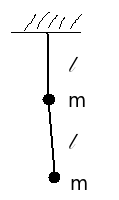
\includegraphics[width=0.6in]{shuangbai.png}
\end{minipage}
\begin{minipage}{0.5\textwidth}
{\scriptsize
如图,在一个长度为$\ell$,质量为$m$的理想刚性单摆下再悬挂一个相同的单摆。节点处都认为可以无阻力自由在所示的平面内转动。本地重力常数为$g$。试求该系统的量子零点能。}
\end{minipage}


{\scriptsize
解答:仅考虑小幅振动。取两个质点的横向位移分别为$x_1$, $x_2$。则垂直位移分别为 $\frac{x_1^2}{2\ell}$和$\frac{x_1^2}{2\ell} + \frac{(x_2-x_1)^2}{2\ell}$,系统的拉氏量为
$$L = \frac{m}{2}\left(\dot{x}_1^2 + \dot{x}_2^2\right) - \frac{mg}{2\ell}\left[2x_1^2+(x_2-x_1)^2\right] = \frac{m}{2}\dot{\vecx}^T \dot{\vecx}-\frac{1}{2}m \vecx^T \Omega^2 \vecx$$
其中
\be
\vecx = \left( \begin{array}{l} x_1 \\ x_2 \end{array} \right),\ 
\Omega^2 = \frac{g}{\ell}\left( \begin{array}{rr} 3 & -1 \\ -1 & 1 \end{array}\right) \,.
\ee
假设$\Omega^2$的本征值为$\omega_1^2$和$\omega_2^2$,则$\omega_1^2+\omega_2^2 = \trof{\Omega^2} = 4\frac{g}{\ell}$, $\omega_1^2\omega_2^2 = \det{(\Omega^2)} = 2\frac{g^2}{\ell^2}$。所以真空能$E_{\rm vac} = \frac{1}{2}(\omega_1+\omega_2) = \frac{1}{2}\sqrt{\omega_1^2+\omega_2^2 + 2\sqrt{\omega_1^2\omega_2^2}} =\frac{1}{2}\sqrt{\left(4+2\sqrt{2}\right)\frac{g}{\ell}}$
}

\ech
\end{frame}

\begin{frame}
\chtitle{第3题 奇怪的一维量子场}
\bch
\begin{minipage}{0.3\textwidth}
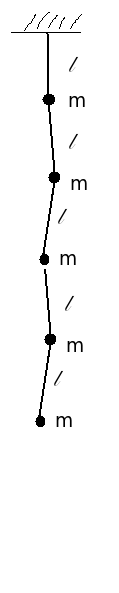
\includegraphics[width=0.32in]{duobai.png}
\end{minipage}
\begin{minipage}{0.5\textwidth}
{\scriptsize
把上题推广到$N$个长度为$\ell$,质量为$m$的理想刚性单摆首位连接挂起来(如左图给出了一个$N=5$的例子),所有的单摆都可以无摩擦在所示的平面内转动。记系统的总量子零点能为$E_N$。当$N\rightarrow \infty$时,$E_N/N^{3/2}$趋向于一个常数,试计算这个常数(用$\ell$, $g$, $m$来表示)。
}
\end{minipage}

{\scriptsize
解答:如上题一样设$N$个质点的横向位移分别为$x_1$, $x_2$, $\ldots$, $x_N$。把拉氏量写为
$$L = \frac{m}{2}\dot{\vecx}^T \dot{\vecx}-\frac{1}{2}m \vecx^T \Omega^2 \vecx$$
其中
{\tiny
\be
\vecx = \left( \begin{array}{l} x_1 \\ x_2 \\ . \\ . \\ . \\ x_N  \end{array} \right),\ 
\Omega^2 = \frac{g}{\ell}\left( \begin{array}{cccccccc} 2N-1 & -(N-1) & & & & & \\ -(N-1) & 2N-3 & -(N-2) & & & & & \\  & -(N-2) & 2N-5 & -(N-3) & & & & \\ & &  & & \ldots & & & \\ & & & & & -2 & 3 & -1 \\ & & & & & & -1 & 1 \end{array}\right) \,.
\ee
}
}
\ech
\end{frame}

\begin{frame}
\chtitle{第3题解答续}
\bch
{\tiny
于是问题转化为求解$\Omega^2$的本征值$\omega_1^2$, $\omega_2^2$, $\ldots$, $\omega_N^2$。

我们先忘掉原问题,考虑一个相对较简单的矩阵的本征值问题,对$n\in Z$,定义一个$n \times n$ 的矩阵
\be
S_n = \left( \begin{array}{cccccccc} 2 & -1 & & & & & \\ -1 & 2 & -1 & & & & & \\  & -1 & 2 & -1 & & & & \\ & &  & & \ldots & & & \\ & & & & & -1 & 2 & -1 \\ & & & & & & -1 & 2 \end{array}\right) 
\ee
取变量$\vecx = (x_0, x_1, \ldots, x_{n-1})^T$,则$S_n$对应的二次型耦合谐振子系统的势能可以写为
$$ \frac{1}{2}\vecx^T S_n\vecx =  \frac{1}{2}\left[(x_0-x_1)^2 + (x_1-x_2)^2 + \ldots + (x_{n-2}-x_{n-1})^2\right]$$
为了使上式有周期对称性,我们给上述势能加上一项 $\frac{1}{2}(x_0-x_{n-1})^2$,并(不加证明地,厚颜无耻地)认为当$n \rightarrow \infty$时这样加一项造成的影响可以忽略。
$$\vecx^T S_n\vecx \approx \sum_{i=0}^{n-1} (x_i-x_{i+1})^2$$
其中我们约定符号$x_n = x_0$。
}
\ech
\end{frame}

\begin{frame}
\chtitle{第3题解答续}
\bch
{\tiny
现在我们取离散傅立叶变换
\be
y_i \equiv \frac{1}{\sqrt{n}}\sum_{j=0}^{n-1} x_j e^{-\frac{2\pi i j}{n} \ii} 
\ee
其逆变换为
\be
x_i = \frac{1}{\sqrt{n}} \sum_{j=0}^{n-1}y_j e^{\frac{2\pi i j}{n} \ii} 
\ee
上式的证明如下:
\bea
 \frac{1}{\sqrt{n}} \sum_{j=0}^{n-1}y_j e^{\frac{2\pi i j}{n} \ii}
&=& \frac{1}{n} \sum_{j=0}^{n-1}\sum_{k=0}^{n-1}x_k e^{\frac{2\pi (i-k)j}{n} \ii} \newl
&=& \frac{1}{n} \sum_{k = i} x_k \sum_{j=0}^{n-1} e^{\frac{2\pi (i-k)j}{n} \ii}  + \frac{1}{n} \sum_{k\ne i} x_k \sum_{j=0}^{n-1} e^{\frac{2\pi (i-k)j}{n} \ii} \newl
&=& \frac{1}{n} x_i \sum_{j=0}^{n-1} 1  + \frac{1}{n} \sum_{k\ne i} x_k \frac{1-e^{\frac{2\pi (i-k)n}{n} \ii}}{1-e^{\frac{2\pi (i-k)}{n} \ii}} \newl
&=& x_i + 0 \newl
&=& x_i
\eea
不难验证,上述逆变换公式对$i=n$的情况也会正确地给出$x_n = x_0$,或更一般地可以拓宽下标的范围:$x_{n+i} = x_i$,$y_{n+i} = y_i$。
}
\ech
\end{frame}


\begin{frame}
\chtitle{第3题解答续}
\bch
{\tiny
此外,我们还可以验证离散傅立叶变换是保持矢量模不变的幺正变换,即
\be
\sum_{i=0}^{n-1} |y_i|^2 = \sum_{i=0}^{n-1} |x_i|^2
\ee
上式证明如下:
\bea
\sum_{i=0}^{n-1} |x_i|^2 &=& \sum_{i=0}^{n-1} x_i^*x_i \newl
&=& \sum_{i=0}^{n-1} \frac{1}{n}\sum_{j=0}^{n-1} y_j^* e^{-\frac{2\pi i j}{n} \ii} \sum_{k=0}^{n-1} y_ke^{\frac{2\pi i k}{n} \ii} \newl
&=& \sum_{j=0}^{n-1}\sum_{k=0}^{n-1} y_j^*y_k \frac{1}{n} \sum_{i=0}^{n-1}  e^{\frac{2\pi i (k-j)}{n} \ii}  \newl
&=& \sum_{j=0}^{n-1}\sum_{k=0}^{n-1} y_j^*y_k \delta_{jk} \newl
&=& \sum_{j=0}^{n-1} |y_j|^2 
\eea
}
\ech
\end{frame}


\begin{frame}
\chtitle{第3题解答续}
\bch
{\tiny
利用
\be
x_i = \frac{1}{\sqrt{n}} \sum_{j=0}^{n-1}y_j e^{\frac{2\pi i j}{n} \ii} 
\ee
即得到
\be
x_i - x_{i+1} = \frac{1}{\sqrt{n}} \sum_{j=0}^{n-1}y_j\left(1-e^{\frac{2\pi j}{n}\ii}\right) e^{\frac{2\pi i j}{n} \ii} 
\ee
定义 $z_j \equiv y_j\left(1-e^{\frac{2\pi j}{n}\ii}\right)$,则由上式可以看出$z_0$, $z_1$, $\ldots$, $z_{n-1}$是$x_0-x_1$, $x_1-x_2$, $\ldots$, $x_{n-1}-x_{n}$的离散傅立叶变换。根据离散傅立叶变换保持模不变的性质,即有
$$\sum_{i=0}^{n-1} (x_i-x_{i+1})^2 = \sum_{i=0}^{n-1} |z_i|^2 = \sum_{i=0}^{n-1} 4\sin^2{\frac{\pi i}{n}} |y_i|^2  $$
也就是说,原先势能为$\frac{1}{2}\vecx^T S_n \vecx$的耦合谐振子,经过离散傅立叶变换可以对角化为频率分别为$2\sin{\frac{\pi i}{n}}$ ($i= 0, 1, \ldots, n-1)$的独立谐振子(模仿课上对实标量场进行对角化的最后一步,把$y$进行实,虚步分离,可以化为标准的谐振子形式)。所以我们得到$S_n$的频谱为
$\omega_i = 2\sin{\frac{\pi i}{n}}$ ($i=0,1,2,\ldots, n-1$)。其每个自由度的平均频率在$n\rightarrow\infty$的极限下为
$$\bar{\omega} =  \frac{\int_0^\pi 2\sin x \,dx}{\int_0^\pi dx} = \frac{4}{\pi}$$ 

}
\ech
\end{frame}


\begin{frame}
\chtitle{第3题解答续}
\bch
{\tiny
最后我们回到原问题,当$N$很大时,我们取$N = n p$ 并令$p \gg n \gg 1$。

我们再次(不加证明地,厚颜无耻地)把$\frac{l}{g}\Omega^2$“近似”为
\bea
\frac{\ell}{g}\Omega^2 \approx \left(
\begin{array}{llllll}
pn S_n  & & & & & \\ 
& (p-1)n S_n  & & & &  \\ 
& & (p-2)n S_n  & & & \\ 
& &  & \ldots & & \\ 
& &  &  & 2n S_n & \\ 
& &  &  &  & n S_n\\ 
\end{array}
\right) \, .
\eea
根据前面对$S_n$的讨论可知,$kn S_n$的平均本征频率为$\frac{4}{\pi}\sqrt{kn}$ ,即本征频率之和为$\frac{4n^{3/2}}{\pi}\sqrt{k}$ ($k=1, 2, \ldots, p$)。
所以$\frac{l}{g}\Omega^2$的本征频率之和为
$ \frac{4n^{3/2}}{\pi} \sum_{k=1}^p \sqrt{k} \approx \frac{4n^{3/2}}{\pi} \int_0^p \sqrt{k} = \frac{8n^{3/2}}{3\pi}p^{3/2} = \frac{8}{3\pi}N^{3/2} $

即$N\rightarrow \infty$时,
$$E_N/N^{3/2} \rightarrow \frac{4}{3\pi}\sqrt{\frac{g}{\ell}}$$

}
\ech
\end{frame}


\begin{frame}
\chtitle{第4题 环上的量子场}
\bch
{\scriptsize 假设“脑洞大开世界”为一个一维圆环加上一维时间,时空度量元为
$$ds^2 = dt^2 - R^2 d\theta^2$$
其中$R>0$为固定常数,$(t,\theta)$为时空坐标。在这个时空里的质量为$m$的实标量场$\phi(t,\theta)$满足周期性边界条件
$$\phi(t,\theta+2\pi) = \phi(t,\theta)$$
其自由场拉氏量为
$$L_{\rm free} = \int_0^{2\pi}d\theta\ \frac{1}{2}\left[\left(\frac{\partial\phi}{\partial t}\right)^2-\frac{1}{R^2}\left(\frac{\partial\phi}{\partial\theta}\right)^2-m^2\phi^2\right]$$
试把$\phi$场量子化。
}
\ech
\end{frame}

\begin{frame}
\chtitle{第4题解答}
\bch
{\scriptsize
解答:由周期性边界条件可以把$\phi$展开为
$$\phi = \sum_{k=-\infty}^{\infty} \phi_k e^{\ii k\theta}$$
且由$\phi$为实数可以得到$\phi_{-k} = \phi^*_k$。
可以仿照课上对实标量场的量子化方法把$\phi$量子化(过程略),唯一的区别是动量$k$为离散的整数值。
}
\ech
\end{frame}


\begin{frame}
\chtitle{第5题 环上的量子场的散射}
\bch
{\scriptsize
给上题中的场$\phi$加一个自相互作用的拉氏量,
$$L = L_{\mathrm{free}} - \int_0^{2\pi}d\theta\ \frac{\lambda}{4!}\phi^4$$
其中$\lambda\ll 1$为耦合常数。

试证明,这个场的两个粒子不可能发生散射变成和初态不同的两个粒子。
}

\skipline

{\scriptsize
解答:设散射初态动量为$p_1$, $p_2$,末态动量为$p_3$, $p_4$。因为是一维的情况,由能量动量守恒即知道$p_3$, $p_4$必须和$p_1$,$p_2$相同。
}
\ech
\end{frame}


\end{document}
